\documentclass{article}

\usepackage{amsmath,amssymb}
\usepackage{fullpage}
\usepackage{enumerate}
\usepackage{hyperref}
\usepackage{graphicx}

\begin{document}

\begin{center}
\textbf{\Large Intermediate Monthly Problem Set}
\\ \vspace{1em}
\textbf{\large Due: Friday, 17 January 2020}
\end{center}

\begin{enumerate}[1.]

\vspace{6pt}
\item % 1994 talent search
Find all integers $m$ and $n$ such that $5m- 7n = 1$.

\vspace{6pt}
\item %1995 talent search
Prove that, if $a, b$ and $c$ are positive numbers such that $a < b + c$, then
\begin{center}
	$\frac{a}{1+a} < \frac{b}{1+b} + \frac{c}{1+c}$
\end{center}

\vspace{6pt}
\item
In the figure, $BC = CA$, $EC = CD$ and $\angle BCA$ = $\angle DCE = 90^{\circ}$. If $P, Q, R$ and $S$ are the
midpoints of $AB, BD, DE$ and
$EA$ respectively, prove, in two
different ways, that $PQRS$ is a
square.
\begin{center}
	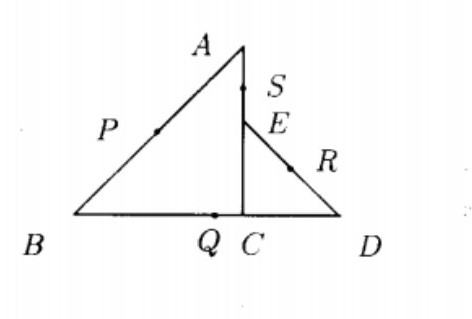
\includegraphics[scale=0.5]{int_q5.jpg}
\end{center}


\item % 1995 talent search
Prove that among any six integers there will be a pair whose sum
or difference is divisible by 9.

\vspace{6pt}
\item %1995 booklet talent search
Prove that, if $a, b$ and $c$ are positive numbers such that $abc= 1$, then
\begin{center}
	$\frac{a}{ab + a + 1} + \frac{b}{bc + b + 1} + \frac{c}{ca + c + 1} = 1$
\end{center}

\vspace{6pt}
\item 
$\triangle ABC$ and $\triangle DBE$ are isosceles with $\angle ABC = \angle DBE = 36^{\circ}$ and $AB = BC$ and $DB = DE$. Find the angle between lines $AD$ and $CE$.

\vspace{6pt}
\item  %PAMO Shortlist 2019
On the board, we write the integers $1, 2, 3, \dots, 2019$. At each minute, we pick two numbers on the board $a$ and $b$, erase them, and write down the number $s(a + b)$ instead where $s(n)$ denotes the sum of the digits of the integer $n$. Let $N$ be the last number remaining on the board.
\begin{enumerate}
	\item Is it possible that $N = 19$?
	\item Is it possible that $N = 15$?
\end{enumerate}

\vspace{6pt}
\item  %Baltic Way 2009 Problem 8
For which positive integers $n$ is it possible to divide the numbers $n, (n + 1), (n + 2), \dots, (n + 8)$ into two disjoint sets $A$ and $B$ such that the product of the numbers in $A$ is equal to the product of the numbers in $B$?

\end{enumerate}


\vspace{4pt}
\textbf{\Large Email submission guidelines}
\begin{itemize}
	\item Email your solutions to \href{mailto:samf.training.assignments@gmail.com}{\texttt{samf.training.assignments@gmail.com}}.
	\item In the subject of your email, include your name and the level of the assignment (Beginner, Intermediate or Senior).
	\item Submit each question in a single separate PDF file (with multiple pages if necessary), with your name and the question number written on each page.
	\item If you take photographs of your work, use a document scanner such as Office Lens to convert to PDF.
	\item If you have multiple PDF files for a question, combine them using software such as PDFsam.
\end{itemize}

\end{document}